% ============================================================
%  Capítulo 3: Dados e análise exploratória
% ============================================================

\chapter{Dados e análise exploratória}
\label{cap:material}
\raggedbottom

O Capítulo~\ref{cap:metodologia} apresentou os métodos. Este capítulo mostra os dados a que eles se aplicam, na ordem em que foram preparados: a base, o painel no formato \textit{start--stop} da Seção~\ref{subsec:cox_vdt}, a escolha e o tratamento das covariáveis, o que cada modelo recebe e a análise exploratória.

% ─────────────────────────────────────────────────────────────
\section{A base de dados}
\label{sec:contexto}

Os dados vêm do conjunto público de \citet{hyde_nflstats}, montado com uma biblioteca em Python \citep{nfldatapy} que lê dados do ecossistema \textit{nflverse} \citep{nflverse}, na versão com temporadas de 2012 a 2024. A base de estatísticas ofensivas por temporada tem 7.133 linhas e 660 colunas, de 2012 a 2024. Cada linha é um jogador em um time em uma temporada. São 6.150 linhas de temporada regular e 983 de pós-temporada, em 18 posições. O estudo usa cinco grupos de variáveis: desempenho, uso e oportunidade, recrutamento e físico, disponibilidade e carreira na janela.

Ficam de fora a pós-temporada, que só as equipes classificadas disputam, e as demais posições. As 4.602 linhas de temporada regular de QB, RB e WR se consolidam em 4.473 pares jogador-temporada de 1.151 jogadores (Tabela~\ref{tab:amostra}). A soma por posição é de 1.152 porque um jogador aparece nos painéis de RB e de WR.

\begin{table}[H]
\centering
\caption{Amostra por posição, 2012--2024: jogadores, temporadas (linhas jogador-temporada do painel), saídas, censurados e percentual de censura.}
\label{tab:amostra}
\thesistablesetup
\begin{tabular*}{\textwidth}{@{\extracolsep{\fill}}lccccc@{}}
\toprule
\textbf{Posição} & \textbf{Jogadores} & \textbf{Temporadas} & \textbf{Saídas} & \textbf{Censurados} & \textbf{Censura (\%)} \\
\midrule
QB  & 182 & 848  & 107 & 75  & 41{,}2\% \\
RB  & 397 & 1.454 & 289 & 108 & 27{,}2\% \\
WR  & 573 & 2.171 & 394 & 179 & 31{,}2\% \\
\bottomrule
\end{tabular*}
\end{table}

% ─────────────────────────────────────────────────────────────
\section{Da base ao painel}
\label{sec:tratamentos_eda}

A base traz uma linha por jogador, time e temporada, mas a análise de sobrevivência precisa acompanhar cada jogador ao longo da carreira. A unidade do painel é, por isso, o par jogador-temporada. Quando um jogador atua em dois times na mesma temporada, as duas linhas viram uma, e as estatísticas de temporada recebem o máximo entre as passagens (Apêndice~\ref{apx:multitime}). Cada jogador fica com uma linha por temporada, no formato \textit{start--stop} de processo de contagem \citep{andersen1982}, e o tempo é a experiência acumulada na NFL, não o número de temporadas observadas entre 2012 e 2024.

Cada linha tem ao menos um jogo ou um \textit{snap} ofensivo. A base não registra a saída da liga: ela é reconhecida pela falta de temporadas seguintes. Jogos perdidos são 16 ou 17 menos os jogos disputados, sem separar lesão, banco ou corte. Uma temporada sem jogar nem sempre é definitiva, já que, entre 2013 e 2023, 182 de 872 ausências (21\%) foram seguidas de retorno. Por isso, quem volta segue na mesma carreira, e só a última temporada conta como saída. Quem ainda joga em 2024 não tem saída observada e é censurado. As saídas de 2023 só se confirmam pela ausência em 2024. Como a janela começa em 2012, quem já jogava antes entra no conjunto de risco com a experiência que tinha. A Tabela~\ref{tab:decisoes} reúne essas regras, detalhadas no Apêndice~\ref{apx:regras_painel}.

\begin{table}[H]
\centering
\caption{Regras do painel: como se definem o evento (saída), o retorno, a censura e a entrada tardia de cada jogador.}
\label{tab:decisoes}
\thesistablesetup
\begin{tabularx}{\textwidth}{@{}>{\raggedright\arraybackslash}p{3.3cm}Y@{}}
\toprule
\textbf{Decisão} & \textbf{Regra} \\
\midrule
Evento (saída da liga) & A última temporada regular do jogador na liga, quando ela é anterior a 2024; a saída é tratada como ocorrida ao fim dessa temporada. \\
\addlinespace
Retorno & Ausência seguida de retorno é continuação da mesma carreira. \\
\addlinespace
Troca de posição & Censura ao sair do painel da posição, sem evento. \\
\addlinespace
Censura em 2024 & Quem joga em 2024 é censurado à direita: sem a temporada de 2025 na base, não há como saber se ele saiu. \\
\addlinespace
Entrada tardia & Quem já jogava antes de 2012 entra com \textit{start} $>0$. \\
\bottomrule
\end{tabularx}
\end{table}

% ─────────────────────────────────────────────────────────────
\section{Das 660 colunas ao conjunto de covariáveis}
\label{sec:covariaveis}

Das 660 colunas da base, a escolha por conhecimento do jogo chega às variáveis que um gerente geral olha ao decidir sobre um jogador. Elas formam os cinco grupos da Tabela~\ref{tab:grupos}, com listas próprias por posição, porque os mesmos sinais não medem o mesmo em um QB, um RB ou um WR. Esse conjunto é o ponto de partida dos dois ramos de análise.

\begin{table}[H]
\centering
\caption{Conjunto de covariáveis do painel por grupo e posição: exemplos de cada grupo e número de covariáveis.}
\label{tab:grupos}
\thesistablesetup
\begin{tabularx}{\textwidth}{@{}>{\raggedright\arraybackslash}p{2.9cm}Yccc@{}}
\toprule
\textbf{Grupo} & \textbf{Exemplos} & \textbf{QB} & \textbf{RB} & \textbf{WR} \\
\midrule
Desempenho & Eficiência de passe (QB), profundidade dos alvos (WR), taxas de carreira e seus indicadores de dado faltante & 11 & 4 & 9 \\
\addlinespace
Uso e oportunidade & Profundidade no elenco, participação ofensiva, fatia da equipe & 3 & 4 & 3 \\
\addlinespace
Recrutamento e físico & Posição no \textit{draft}, não draftado, idade, altura, peso & 5 & 5 & 5 \\
\addlinespace
Disponibilidade & Jogos perdidos, hiato acumulado na janela, hiato anterior & 3 & 3 & 3 \\
\addlinespace
Carreira na janela & Volumes acumulados, experiência, veterano pré-janela, anos sem estatísticas & 20 & 20 & 19 \\
\midrule
\textbf{Total} & & \textbf{42} & \textbf{36} & \textbf{39} \\
\bottomrule
\end{tabularx}
\end{table}

As covariáveis têm dois tempos. As da temporada, como jogos perdidos e fatia da equipe, descrevem a temporada $t$. As de carreira acumulam até $t-1$, dentro de 2012--2024, e por isso nunca incluem a produção da própria temporada. Como essa janela não enxerga o que veio antes de 2012, três variáveis marcam quem tem história fora dela. O indicador de veterano pré-janela, com carreira iniciada antes de 2012, vale para 53 QBs, 79 RBs e 108 WRs. O indicador de primeira linha com anos sem estatísticas marca 82 QBs, 111 RBs e 181 WRs, grupo que inclui veteranos e também draftados a partir de 2012 cuja primeira estatística é posterior à entrada, e um contador guarda esses anos. O glossário completo está no Apêndice~\ref{apx:glossario}.

% ─────────────────────────────────────────────────────────────
\section{Tratamento das covariáveis}
\label{sec:selecao_faltantes}

Antes dos modelos, o conjunto passa por dois tratamentos: o dos dados faltantes e o das redundâncias.

\subsection{Dados faltantes}
\label{subsec:imputacao}

Aqui, um dado faltante é, quase sempre, algo que não existe para medir. O caso principal são as taxas de carreira, como o percentual de passes completos e a taxa de recepção: com denominador de até 50 oportunidades, a taxa não é calculada, e isso atinge 30\% a 52\% das linhas do QB, 41\% das do RB e 46\% a 55\% das do WR, sobretudo novatos. Há ainda 26 linhas do QB sem tentativa de passe, nas quais a eficiência não existe, e os não draftados, que não têm posição no \textit{draft}. Descartar essas linhas tiraria justamente o início das carreiras, onde muitas saídas acontecem, e os modelos exigem uma matriz completa.

A regra adotada preenche o valor com uma mediana. Nas taxas de carreira, usa-se a do grupo de anos de experiência $g(i)$ do jogador, $m_{j,g}$, com a mediana global $m_j$ como reserva; nas demais, $m_j$:
\begin{equation}
    \tilde{x}_{ij} = \begin{cases} x_{ij}, & \text{se observado}, \\ m_{j,g(i)}, & \text{se ausente e $x_j$ é taxa de carreira}, \\ m_j, & \text{se ausente nas demais}. \end{cases}
    \label{eq:missing}
\end{equation}
Cada taxa com dado faltante ganha também um indicador binário, $I_{ij} = \mathbf{1}(x_{ij} \text{ ausente})$, que na inferência concorre na seleção como as demais covariáveis. Os não draftados recebem indicador igual a 1 e posição igual a zero, de modo que, quando o indicador está no modelo, o efeito de não ser draftado fica todo nele. Na predição, as medianas e a padronização são ajustadas só no treino de cada origem. Na inferência, a amostra da posição é o conjunto de ajuste, e os HR são lidos por desvio-padrão da covariável.

Essa regra foi comparada a quatro alternativas: limiares de 25 a 100 oportunidades, zero ou exclusão no lugar da mediana na eficiência, imputação múltipla com o desfecho e outras codificações dos não draftados. A seleção do QB não muda com a codificação, a do RB e a do WR mudam; o HR da eficiência fica entre 0,60 e 0,65, e a imputação múltipla não altera nenhuma conclusão (Apêndices~\ref{subsec:imputacao_apend} e~\ref{apx:undrafted}).

\subsection{Colinearidade}
\label{subsec:triagem_colinearidade}

Muitas covariáveis medem quase a mesma coisa, e isso impede separar o efeito de cada uma. No QB, as jardas e as tentativas de passe acumuladas até $t-1$ têm $r=0{,}998$; no RB, os alvos e as recepções acumulados têm $r=0{,}997$, e a fatia de tentativas e a fatia de jardas terrestres têm $r=0{,}988$. Pares com correlação de Pearson acima de um limiar $c = 0{,}85$ são tratados como redundantes,
\begin{equation}
    |\rho_{jl}| > c,
    \label{eq:colinearidade}
\end{equation}
e a remoção é gulosa: a cada passo sai a covariável com mais pares acima de $c$, até nenhum par ultrapassar o limiar. O filtro não avalia os indicadores de dado faltante. O filtro roda em cada ramo com seus próprios dados; a escolha da janela no ramo preditivo é testada no Apêndice~\ref{subsec:apend_janela_x}.

% ─────────────────────────────────────────────────────────────
\section{Dois ramos: inferência e predição}
\label{sec:dois_empregos}

O painel posicional, com 42 covariáveis no QB, 36 no RB e 39 no WR, alimenta as duas análises, que chamamos de ramos. Os dois ramos seguem as duas culturas de modelagem de \citet{breiman2001cultures}: a inferência supõe um modelo para os dados e lê os seus parâmetros, e a predição trata o mecanismo como desconhecido e é julgada pela acurácia em dados que o ajuste não viu. Como as perguntas são diferentes, cada ramo seleciona de um jeito: a inferência busca uma lista parcimoniosa dos preditores mais importantes, para ler os HR e os $B_j(t)$ com clareza, e a predição usa o painel sem seleção por valor-$p$, com o mesmo conjunto para os modelos comparados \citep{harrell2001}.

\subsection{Ramo inferencial}
\label{sec:prep_inferencia}

A seleção é feita na janela 2012--2024. No Cox, uma covariável só pode ser estimada se variar entre os jogadores em risco no mesmo tempo, porque a verossimilhança parcial compara apenas quem está em risco em cada saída. Duas colunas não cumprem isso e são retiradas, por não serem identificáveis. A experiência é o próprio tempo, igual para todos em cada conjunto de risco (Apêndice~\ref{subsec:apend_years_exp}). A primeira temporada observada é constante no primeiro ano e, a partir do segundo, repete o indicador de histórico não observado dentro de cada conjunto de risco. Sem essas colunas e sem indicadores duplicados, sobram 37, 33 e 35 candidatas. O filtro de colinearidade reduz o conjunto para 26, 20 e 25. Somam-se os indicadores das taxas selecionadas, e a revalidação da identificabilidade deixa 23, 19 e 23 candidatas, de onde cada modelo parte com seu critério.

\label{subsec:selecao_cox}
\textbf{Cox.} A eliminação retroativa (\textit{backward stepwise}) parte do modelo com todas as candidatas, passa pelo ajuste completo e é preferível à seleção progressiva \citep{harrell2001}. A cada passo, sai a covariável de maior valor-$p$ na estatística de Wald~\eqref{eq:wald}, e o processo para quando todas têm $p<0{,}05$: 5, 5 e 7. As candidatas, em conjunto, separam-se do modelo nulo nas três posições ($p<0{,}001$), e a lista final não perde ajuste contra o modelo com todas elas: $p = 0{,}793$ no QB, $0{,}782$ no RB e $0{,}620$ no WR. A lista foi escolhida nesses mesmos dados, e por isso esse teste é descritivo; a estabilidade da seleção está no Apêndice~\ref{subsec:apend_frequencia}.

\textbf{Aalen.} Cada candidata é testada isoladamente, com a implementação do pacote \texttt{survival} do R, pelo teste de média nula, no trecho de sua própria janela de posto completo, e entra quando $p < 0{,}05$. O Aalen não recebe indicadores de dado faltante, porque exige posto completo, e o ajuste final tem 10, 9 e 13. A triagem univariada ignora a correlação entre covariáveis e pode descartar preditores que só têm efeito em conjunto \citep{harrell2001}.

\textbf{Limite de covariáveis.} Nos dois modelos, a regra de eventos por variável (EPV) \citep{harrell2001} limita o número de covariáveis a
\begin{equation}
    \left\lfloor \frac{E}{10} \right\rfloor,
    \label{eq:epv}
\end{equation}
em que $E$ é o número total de eventos da posição; se restarem mais covariáveis que esse teto, mantêm-se as de menor valor-$p$. É uma heurística de cautela amostral, que pode ser relaxada conforme o contexto \citep{vittinghoff2007}.

\textbf{Cox--Aalen.} Não tem seleção própria: usa a lista final do Cox, e o teste de Schoenfeld de cada covariável, a $5\%$, define o bloco aditivo ou multiplicativo. A lista final do Cox e os principais termos do Aalen estão no Capítulo~\ref{cap:resultados}.

\subsection{Ramo preditivo}
\label{sec:prep_predicao}

O ramo preditivo parte do mesmo painel, com 42, 36 e 39 covariáveis. As duas colunas que a inferência não pode usar voltam aqui: a experiência, porque o tempo passa a ser contado a partir da origem e ela deixa de ser o eixo do modelo, e a primeira temporada observada, que deixa de repetir outro indicador dentro do conjunto de risco. O filtro de colinearidade é ajustado nas temporadas 2012--2017 e fica congelado, para que nenhuma temporada de teste escolha a lista. Com a experiência presente, a idade sai por redundância, com correlação de 0,97, 0,94 e 0,96 entre as duas nessas temporadas. Os indicadores de dado faltante não passam pelo filtro, como na inferência. O resultado tem 25 covariáveis no QB, 21 no RB e 25 no WR, o mesmo $X$ para o Cox com penalização $L_2$, o GBSA e o RSF. Este ramo não tem seleção adicional. A seleção por valor-$p$ serve para ler o efeito de cada covariável; para prever, uma covariável sem significância isolada ainda pode melhorar a ordenação, e cada modelo controla a própria complexidade. No Cox, a penalização $L_2$ encolhe os coeficientes, o que estabiliza covariáveis correlacionadas e dispensa a regra de EPV. O GBSA e o RSF não estimam um coeficiente para cada covariável: a cada divisão, as árvores escolhem entre elas, e por isso os dois modelos lidam bem com muitas covariáveis, mesmo correlacionadas \citep{friedman2001,breiman2001}. A complexidade é controlada, no GBSA, pela taxa de aprendizado e pela subamostragem e, no RSF, pelo sorteio de covariáveis e pelo tamanho das folhas. O Kaplan--Meier não usa covariáveis. A Tabela~\ref{tab:selecao_modelos} resume os critérios dos dois ramos.

\begin{table}[H]
\centering
\caption{Conjunto de covariáveis de cada modelo: critério de escolha e número final de covariáveis por posição.}
\label{tab:selecao_modelos}
\thesistablesetup
\begin{tabularx}{\textwidth}{@{}>{\raggedright\arraybackslash}p{2.9cm}Yccc@{}}
\toprule
\textbf{Modelo} & \textbf{Critério} & \textbf{QB} & \textbf{RB} & \textbf{WR} \\
\midrule
Cox & Eliminação retroativa pelo teste de Wald & 5 & 5 & 7 \\
\addlinespace
Aalen & Triagem univariada, cada candidata em sua janela & 10 & 9 & 13 \\
\addlinespace
Cox--Aalen & Lista final do Cox; aditivo + multiplicativo pelo teste de Schoenfeld & 0 + 5 & 2 + 3 & 2 + 5 \\
\addlinespace
Cox penalizado, GBSA e RSF & Mesmo bloco, sem seleção por valor-$p$ & 25 & 21 & 25 \\
\bottomrule
\end{tabularx}
\end{table}

% ─────────────────────────────────────────────────────────────
\section{Análise exploratória}
\label{sec:eda}

A análise exploratória responde ao segundo objetivo do trabalho: descrever quanto duram as carreiras em cada posição e como essa duração varia com os fatores que um elenco observa. Por isso olhamos, nesta ordem, o tempo até a saída, o recrutamento, o lugar no elenco, a idade e as ausências. Os testes (Kruskal--Wallis, Mann--Whitney e log-rank) resumem diferenças entre grupos, sem ajuste por outras covariáveis, e, como não decidem nada na seleção, não passam por correção para múltiplas comparações.

\subsection{Tempo até a saída}
\label{sec:eda_saida}

A contagem de temporadas observadas entre 2012 e 2024 subestima a carreira. A mediana é de 4 temporadas para QBs e de 3 para RBs e WRs, e 47,3\%, 56,2\% e 56,5\% dos jogadores, respectivamente, têm até três temporadas. Parte da carreira antecede 2012: 29,1\% dos QBs, 19,9\% dos RBs e 18,8\% dos WRs já tinham carreira iniciada antes da janela. Por isso, a medida adequada é a duração até a saída, mostrada por Kaplan--Meier com entrada tardia na Figura~\ref{fig:km_global}.

A mediana de experiência até a saída é de 7 anos para QBs (IC 95\%: 6 a 9), 5 para RBs (IC 95\%: 4 a 5) e 5 para WRs (IC 95\%: 4 a 5). Se os censurados saem do risco no início do último intervalo, RB e WR ficam em 4 (Apêndice~\ref{apx:regras_painel}). Esses valores não se comparam ao tempo médio entre ativos da Seção~\ref{sec:motivacao}, que mede carreiras ainda em curso. Metade dos RBs e dos WRs sai até o quinto ano, e a curva do QB cai de forma mais gradual. Um QB com 4 temporadas observadas pode ter 6 ou 7 anos de experiência, porque parte da carreira ficou antes de 2012.

\begin{figure}[H]
\centering
\paneltag{a}
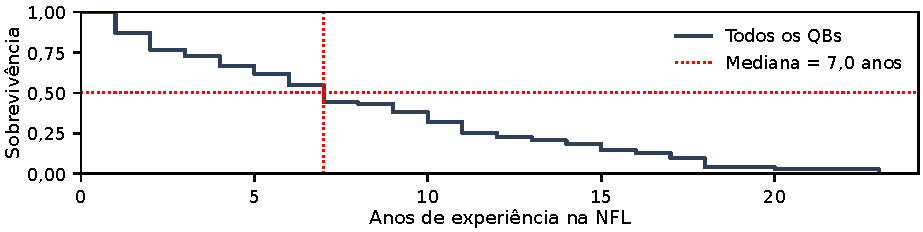
\includegraphics[width=\textwidth,height=0.19\textheight,keepaspectratio]{figuras/km_global_QB.pdf}
\paneltag{b}
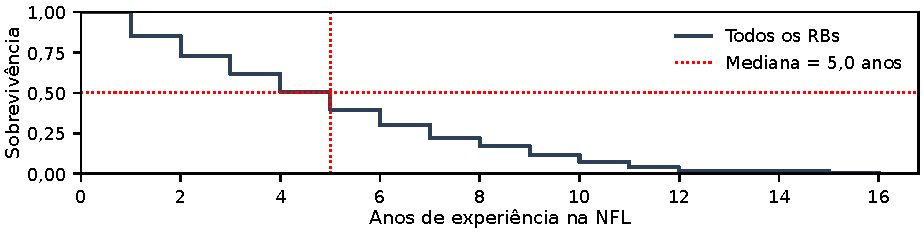
\includegraphics[width=\textwidth,height=0.19\textheight,keepaspectratio]{figuras/km_global_RB.pdf}
\paneltag{c}
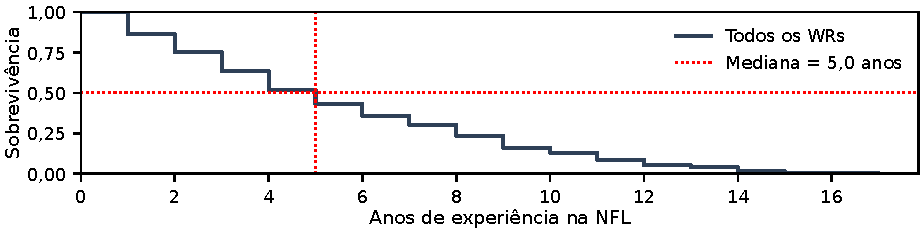
\includegraphics[width=\textwidth,height=0.19\textheight,keepaspectratio]{figuras/km_global_WR.pdf}
\caption[Kaplan--Meier do tempo até a saída, por posição.]{Kaplan--Meier da probabilidade de seguir na NFL (eixo vertical) por anos de experiência (eixo horizontal), por posição. Quem já jogava em 2012 entra na curva com a experiência que tinha (entrada tardia). Linha tracejada: mediana, o tempo em que metade dos jogadores já saiu. \emph{(a)}~QB; \emph{(b)}~RB; \emph{(c)}~WR.}
\label{fig:km_global}
\end{figure}

\subsection{Recrutamento e entrada na liga}
\label{sec:eda_draft}

A posição no \textit{draft} anda com a longevidade nas três posições (Figura~\ref{fig:draft}). Em todas as posições, os selecionados nas rodadas 1 e 2 têm mais temporadas observadas que os não draftados: 5,1 e 4,5 contra 3,1 nos RBs, 4,9 e 4,6 contra 3,3 nos WRs, e 5,5 e 5,8 contra 3,8 nos QBs. No RB e no WR, a média tende a cair ao longo das rodadas, até 2,4 e 2,8 temporadas na rodada 7. No QB, as três primeiras rodadas ficam perto de 5,5 temporadas, e a queda vem na quarta e na quinta, com 3,3 e 2,6. O log-rank das rodadas 1 e 2 contra os não draftados é significativo no RB e no WR ($p<0{,}001$) e não no QB ($p=0{,}45$, com 13 não draftados). Sobre as temporadas observadas, que não corrigem a censura, Kruskal--Wallis rejeita a homogeneidade entre as faixas de \textit{draft} nas três posições ($p=0{,}004$ no QB; $p<0{,}001$ no RB e no WR).

\begin{figure}[H]
\centering
\paneltag{a}
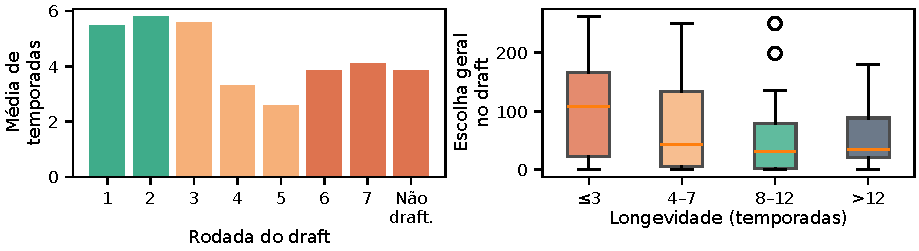
\includegraphics[width=\textwidth,height=0.2\textheight,keepaspectratio]{figuras/draft_QB.pdf}
\paneltag{b}
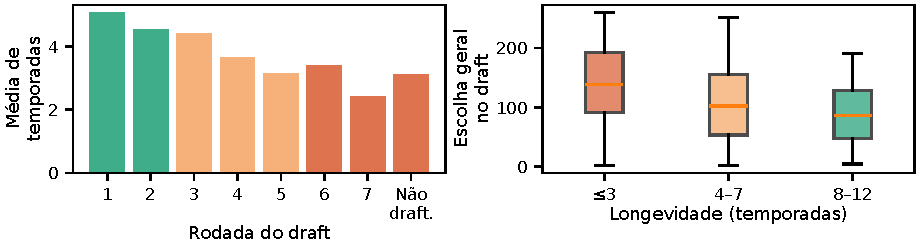
\includegraphics[width=\textwidth,height=0.2\textheight,keepaspectratio]{figuras/draft_RB.pdf}
\paneltag{c}
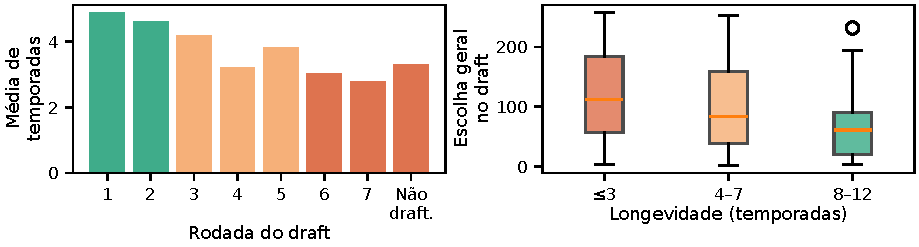
\includegraphics[width=\textwidth,height=0.2\textheight,keepaspectratio]{figuras/draft_WR.pdf}
\caption[Longevidade por faixas de \textit{draft}.]{Esquerda: média de temporadas por rodada do \textit{draft}, com não draftados à parte. Direita: escolha geral no \textit{draft} (quanto menor, mais cedo o jogador foi escolhido) por faixa de longevidade, só entre os draftados. \emph{(a)}~QB; \emph{(b)}~RB; \emph{(c)}~WR.}
\label{fig:draft}
\end{figure}

\subsection{Profundidade no elenco}
\label{sec:eda_profundidade}

A Figura~\ref{fig:depth} mostra, à esquerda, a frequência de cada nível de profundidade no elenco e, à direita, a média desse nível ao longo dos anos de experiência. O titular é o nível mais comum só no QB, com 454 de 848 linhas; no RB e no WR, o segundo nível é o mais frequente, com 640 de 1.454 e 998 de 2.171. A média melhora com a experiência até cerca de nove anos: no RB, de 2,27 na estreia para 1,68 com seis anos, e no WR, de 2,10 para 1,49, enquanto no QB fica perto de 1,5 a 1,6 até cerca de dez anos. Quem é titular no primeiro ano observado permanece mais tempo que reservas e terceiras opções nas três posições (log-rank entre os três grupos, $p<0{,}001$).

\begin{figure}[H]
\centering
\paneltag{a}
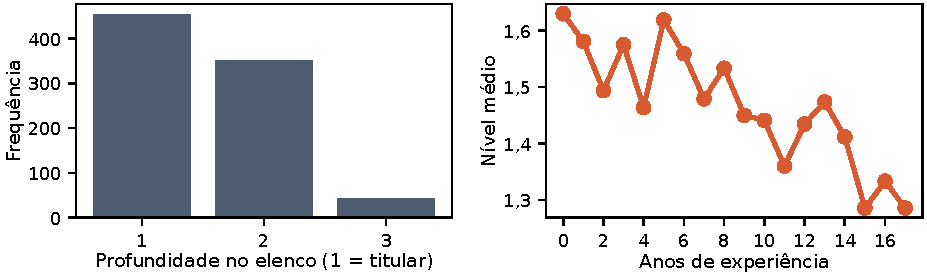
\includegraphics[width=\textwidth,height=0.2\textheight,keepaspectratio]{figuras/depth_QB.pdf}
\paneltag{b}
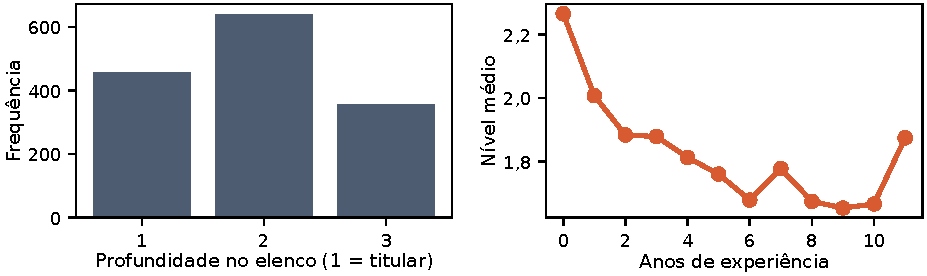
\includegraphics[width=\textwidth,height=0.2\textheight,keepaspectratio]{figuras/depth_RB.pdf}
\paneltag{c}
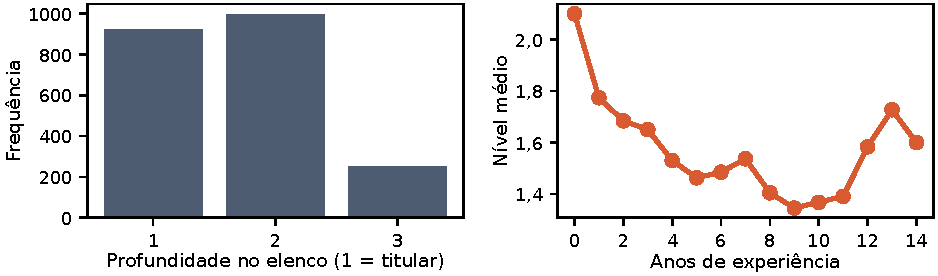
\includegraphics[width=\textwidth,height=0.2\textheight,keepaspectratio]{figuras/depth_WR.pdf}
\caption[Profundidade no elenco, por posição.]{Por posição: à esquerda, frequência de cada nível de profundidade no elenco (1 = titular); à direita, média desse nível por ano de experiência. \emph{(a)}~QB; \emph{(b)}~RB; \emph{(c)}~WR.}
\label{fig:depth}
\end{figure}

\subsection{Idade e jogos perdidos}
\label{sec:eda_outros}

A idade marca sobretudo a entrada tardia, e por isso separa as curvas sem indicar envelhecimento. Entre os jogadores com mais de 25 anos no primeiro ano observado (44 QBs, 34 RBs e 65 WRs), 84\%, 94\% e 94\% já jogavam antes de 2012. Pelo log-rank, a faixa etária separa as curvas nas três posições (QB $p=0{,}030$; RB $p=0{,}013$; WR $p<0{,}001$).

As ausências pedem a mesma atenção: quem fica mais tempo acumula mais jogos perdidos. As medianas de temporadas são de 2 contra 4 no QB, 2 contra 3 no RB e 2 contra 3 no WR, na ordem dos grupos de até 4 e de mais de 4 jogos perdidos em alguma temporada. Também aqui a medida são as temporadas observadas: Mann--Whitney rejeita a igualdade no WR ($p=0{,}002$) e no RB ($p=0{,}048$), não no QB ($p=0{,}169$, com 10 jogadores no grupo de até 4 jogos perdidos).

A Tabela~\ref{tab:eda_testes} reúne os testes da seção. Recrutamento, lugar no elenco e idade separam as durações nas três posições, com uma exceção: o log-rank das rodadas 1 e 2 contra os não draftados no QB. As ausências mostram o limite dessa leitura: sem ajuste, quem perdeu mais jogos dura mais, porque ficou mais tempo exposto. Separar cada fator, com os demais no modelo e a covariável atualizada ano a ano, é o trabalho do Capítulo~\ref{cap:resultados}.

\begin{table}[H]
\centering
\caption{Valores-$p$ dos testes da análise exploratória, que comparam a duração da carreira entre os grupos de cada fator, por posição.}
\label{tab:eda_testes}
\thesistablesetup
\begin{tabular*}{\textwidth}{@{\extracolsep{\fill}}llccc@{}}
\toprule
\textbf{Fator} & \textbf{Teste} & \textbf{QB} & \textbf{RB} & \textbf{WR} \\
\midrule
\textit{Draft} & Log-rank & 0,45 & $<0{,}001$ & $<0{,}001$ \\
\textit{Draft} & Kruskal--Wallis & 0,004 & $<0{,}001$ & $<0{,}001$ \\
Profundidade no elenco & Log-rank & $<0{,}001$ & $<0{,}001$ & $<0{,}001$ \\
Faixa etária & Log-rank & 0,030 & 0,013 & $<0{,}001$ \\
Jogos perdidos & Mann--Whitney & 0,169 & 0,048 & 0,002 \\
\bottomrule
\end{tabular*}
\end{table}
